The general idea is to utilize ParLOT \cite{ parlot} traces for studying HPC application behaviors towards fault detection and localization.
%
%ParLOT
ParLOT collects whole-program function calls and returns at different levels via dynamic binary instrumentation \cite{pin}, and incrementally compresses them on-the-fly.
%
Upon termination of the application, ParLOT flushes out per-thread trace files containing compressed sequence of executed function IDs.
%
The compression mechanism of ParLOT significantly reduces the time, memory and disk overhead, leaves the majority of the system bandwidth for the application. 
%
With the mindset of ``\textit{pay a little upfront to dramatically reduce the number of overall debug iterations}'', ParLOT well overcomes the challenge of whole-program \textit{trace collection} and leaves the \textit{trace analysis} for offline post-mortem analysis, saving HPC resources.
%

% Paragraph about DiffTrace, why we need it and what is our approach?
In this paper, we introduce DiffTrace, a tool-chain that provides an infrastructure for iterative and configurable search space reduction of the HPC whole-program function-call traces, and detection of the most impacted trace(s) and/or region of trace(s).
%
Considering a ``successful’’ termination of the application as \textit{normal behavior}, DiffTrace takes steps towards \textit{abnormal behavior} detection when an application crashes, time outs or produces a corrupted answer.
%
Each abnormal behavior is a potential fault cause or a manifestation of the fault.
%
However, faults in HPC applications may occur or influence the program behavior at different locations and granularities, due to high and hybrid level of parallelism.
%
Also typical HPC applications spend most of their execution time in a main loop until a convergence or over timesteps, and a fault may get  triggered or causing problems after some iteration.
%
Thus accurate automatic fault localization is the problem of finding the needle in a haystack.
%
Due to numerous and comprehensive whole-program function traces, a light-weight single pass of analysis has low chance to reveal interesting facts. A comprehensive heavy analysis also is often not feasible and unpractical.
%
DiffTrace gives the HPC developers the capability of going through the pipeline of trace processing multiple times, each time putting a flash-light on various aspects of the applications' dynamic behavior, gradually collecting evidence about what has happened during execution.
%
\begin{figure}[]
\centering
\caption{Simplified MPI implementation of Odd/Even Sort}
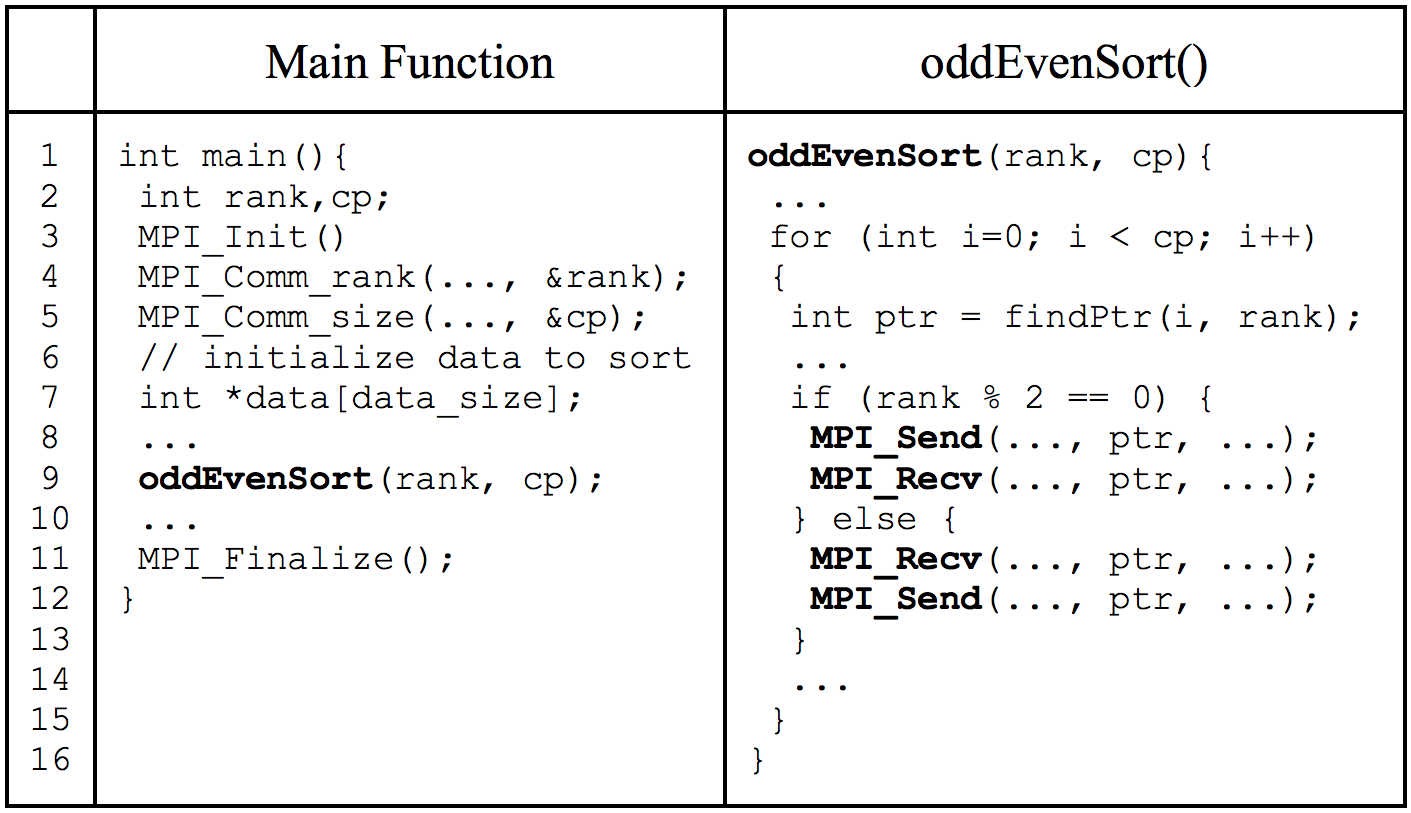
\includegraphics[width=0.45\textwidth]{figs/oddEven.png}
\label{fig.oddEven}
\end{figure}
%
The journey starts from decompressing ParLOT traces and pruning out uninteresting functions from traces. 
%
Loops in source codes reflect themselves as a sequence of \textit{repetitive patterns}, resulting in often-long but redundant traces. A ``nested loop  recognition'' mechanism then mines loops from traces as ``\textit{a measure of progress}'' per thread, and also a loss-less abstraction to ease the rest of trace analysis.
%
The control flow of events in parallel architectures often follow a \textit{regular pattern} such as SPMD, odd-even and master/slave. This characteristic often makes all traces of a single execution tend to fall into just \textit{a few} ``conceptually/behaviorally equivalent classes''.
%
Adopted from the work by Webber et al \cite{weberStructural}, we have applied \textit{formal concept analysis} (FCA)\cite{clbook} techniques to reduce the trace search space into a few classes of traces, and also using the \textit{concept lattice} (CL) data structure as the \textit{model} of execution for further analysis.
%
By comparison of the CL-based models of execution, a ''suspicious candidate table'' is generated for each set of parameters, pointing at traces that have ``changed'' the most after a fault is introduced. 
%
What has changed after a bug is encountered, is visualized by \textit{gdiff}, a graphical representation of differences of a pair of sequences.



Section \ref{sec:components} explains details of DiffTrace components, but before that, we support our ideas over a simple example. 


\begin{figure}[]
\centering
\caption{A line change in oddEvenSort (left) that might cause a deadlock in oddEvenSort\_DL (right)}
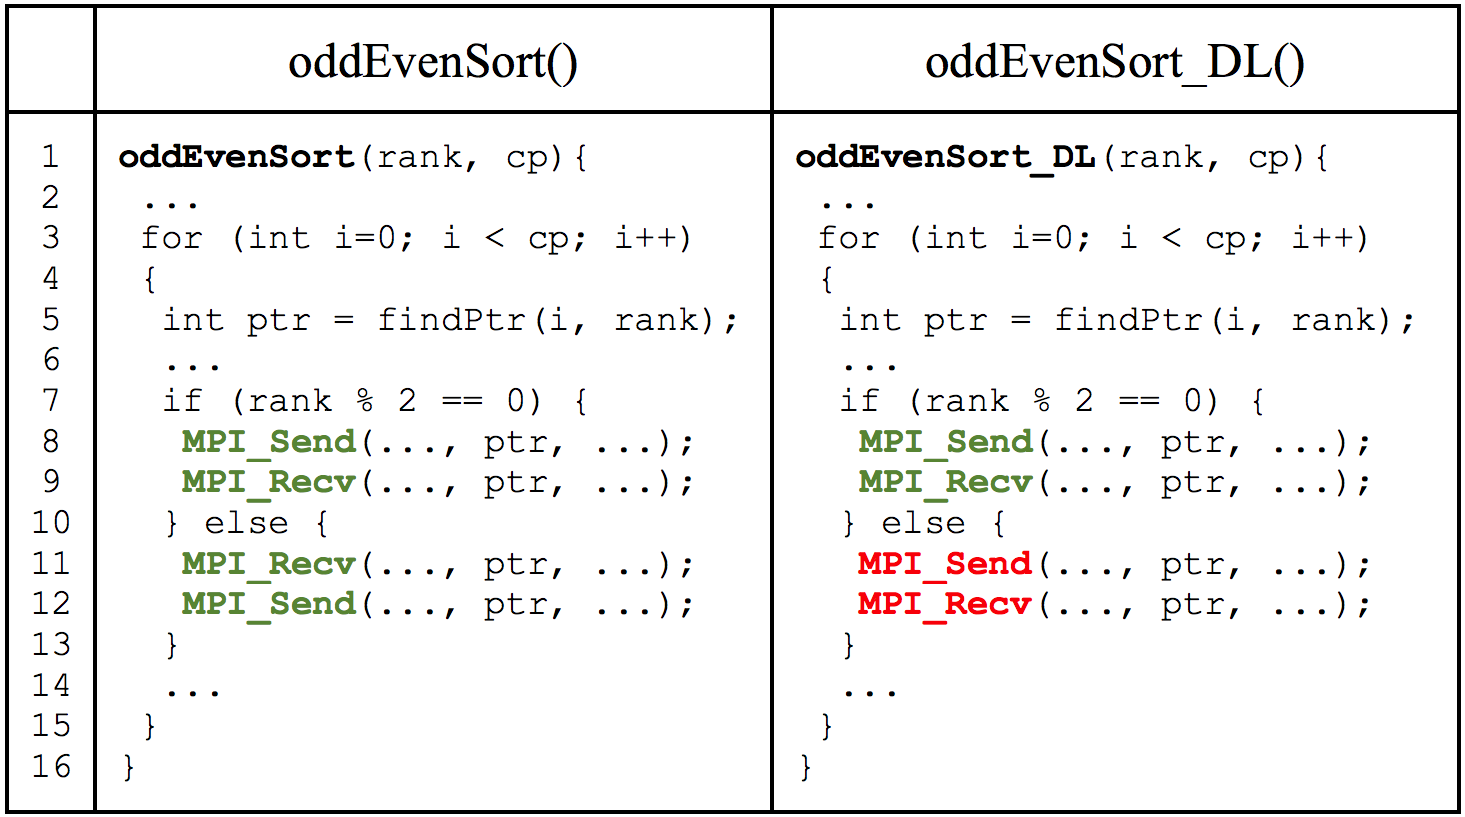
\includegraphics[width=0.45\textwidth]{figs/oddEvenDL.png}
\label{fig.oddEvenDL}
\end{figure}

\subsection{Introducing \textbf{gdiff}: Observing pair-wise differences}
``Diff'' algorithm by Meyers \cite{diff-myers} takes two sequences $S_A$ and $S_B$ and computes the minimal \textit{edit} to convert $S_A$ to $S_B$. This algorithm has been used in GNU \texttt{diff} to compare two text files and in git for efficiently keeping track of file changes.
Since ParLOT preserves the order of function calls in the binary, each per thread trace $T_i$ is totally ordered, thus \textit{diff} can reflect the differences of a pair of $T$s. \textit{gdiff} is the graphical visualization of diff, aligning common and different blocks of a pair of sequences horizontally and vertically, making it easier for analyst to see the differences of a pair of sequences in a glance.  
For simplicity, our implementation of \textit{gdiff} only takes one argument $x$ as \textit{the suspicious trace}

\textit{gdiff}$(x) \equiv $ \textit{gdiff}$(T_x,T_x^\prime)$

where $T_x$ is the trace of thread/process $x$ of a normal/successful execution and $T^\prime_x$ is the corresponding trace of faulty execution.


\subsubsection{gidff via example}
Odd/Even sort is a variant of the bubble-sort operates in two alternate phases: \textit{Phase-even} where even processes exchange (compare and swap) values with right neighbors and \textit{Phase-odd} where odd processes exchange values with right neighbors. Figure \ref{fig.oddEven} shows the simplified MPI implementation of the odd/even sort algorithm.



The for loop in line 4 of \texttt{oddEvenSort()} iterates over phases of the algorithm and based on the phase, the appropriate partner for each rank is getting discovered by the function \texttt{findPtr()} (line 6). The odd/even ranks then exchange their chunks of data (lines 9-13) and a set of sort, merge and copy operations would be performed on received data by each rank (which are replaced by \texttt{...} in line 15 for simplicity).
\\

Execution of odd/even sort application with four processes (\texttt{mpirun -np 4}) while ParLOT trace collection is enabled on top of the application, would result in $T_0$, $T_1$, $T_2$ and $T_3$ (table \ref{tab:oddEvenPT}). This execution terminates successfully with expected results and the set of generated traces clearly reflects the expected behavior (control flow) of odd and even processes.
%


\begin{table}[]
\centering
\caption{The generated PTs for odd/even execution with four processes}
\label{tab:oddEvenPT}
\scalebox{0.75}{
\begin{tabular}{|l|l|l|l|}
\hline
\rowcolor[HTML]{EFEFEF} 
\multicolumn{1}{|c|}{\cellcolor[HTML]{EFEFEF}\textbf{$PT_0$}} & \multicolumn{1}{c|}{\cellcolor[HTML]{EFEFEF}\textbf{$PT_1$}} & \multicolumn{1}{c|}{\cellcolor[HTML]{EFEFEF}\textbf{$PT_2$}} & \multicolumn{1}{c|}{\cellcolor[HTML]{EFEFEF}\textbf{$PT_3$}} \\ \hline \hline
... & ... & ... & ... \\ \\[-1em]  \hline
main & main & main & main \\ \\[-1em]  \hline
MPI\_Init & MPI\_Init & MPI\_Init & MPI\_Init \\ \\[-1em]  \hline
MPI\_Comm\_Rank & MPI\_Comm\_Rank & MPI\_Comm\_Rank & MPI\_Comm\_Rank \\ \\[-1em]  \hline
MPI\_Comm\_Size & MPI\_Comm\_Size & MPI\_Comm\_Size & MPI\_Comm\_Size \\ \\[-1em]  \hline
... & ... & ... & ... \\ \\[-1em]  \hline
oddEvenSort & oddEvenSort & oddEvenSort & oddEvenSort \\ \\[-1em]  \hline
... & ... & ... & ... \\ \\[-1em] \hline
findPtr & findPtr & findPtr & findPtr \\ \hline
\rowcolor[HTML]{FFCCC9} 
{\color[HTML]{333333} MPI\_Send} & \cellcolor[HTML]{CBCEFB}{\color[HTML]{333333} MPI\_Recv} & {\color[HTML]{333333} MPI\_Send} & \cellcolor[HTML]{CBCEFB}{\color[HTML]{333333} MPI\_Recv} \\ \hline
\rowcolor[HTML]{FFCCC9} 
{\color[HTML]{333333} MPI\_Recv} & \cellcolor[HTML]{CBCEFB}{\color[HTML]{333333} MPI\_Send} & {\color[HTML]{333333} MPI\_Recv} & \cellcolor[HTML]{CBCEFB}{\color[HTML]{333333} MPI\_Send} \\ \hline
... & ... & ... & ... \\ \hline
findPtr & findPtr & findPtr & findPtr \\ \hline
\rowcolor[HTML]{FFCCC9} 
{\color[HTML]{333333} MPI\_Send} & \cellcolor[HTML]{CBCEFB}{\color[HTML]{333333} MPI\_Recv} & {\color[HTML]{333333} MPI\_Send} & \cellcolor[HTML]{CBCEFB}{\color[HTML]{333333} MPI\_Recv} \\ \hline
\rowcolor[HTML]{FFCCC9} 
{\color[HTML]{333333} MPI\_Recv} & \cellcolor[HTML]{CBCEFB}{\color[HTML]{333333} MPI\_Send} & {\color[HTML]{333333} MPI\_Recv} & \cellcolor[HTML]{CBCEFB}{\color[HTML]{333333} MPI\_Send} \\ \hline
... & ... & ... & ... \\ \hline
MPI\_Finalize & MPI\_Finalize & MPI\_Finalize & MPI\_Finalize \\ \hline
\end{tabular}}
\end{table}


According to MPI Standard  \hl{[cite MPI-forum or openMPI url]}, MPI\_Send is a \textit{blocking send} used the \textit{standard} communication mode. In this mode,  MPI may buffer outgoing messages and the send call may complete before a matching receive is invoked. On the other hand, buffer space may be unavailable, or MPI may choose not to buffer outgoing messages, for performance reasons. In this case, the send call will not complete until a matching receive has been posted, and the data has been moved to the receiver. This shows that, based on the MPI implementation, the \texttt{oddEvenSort\_DL()} (figure \ref{fig.oddEvenDL}) might end up causing a deadlock, because of the order swap of MPI\_Recv and MPI\_Send in lines 11-12. 
%




\begin{figure}[]
\centering
\caption{(a) The legend of \textit{gdiff} and the list of loop structures (b) \textit{gdiff(5)} of \textit{swapBug} (c) \textit{gdiff(5)} of \textit{dlBug}}
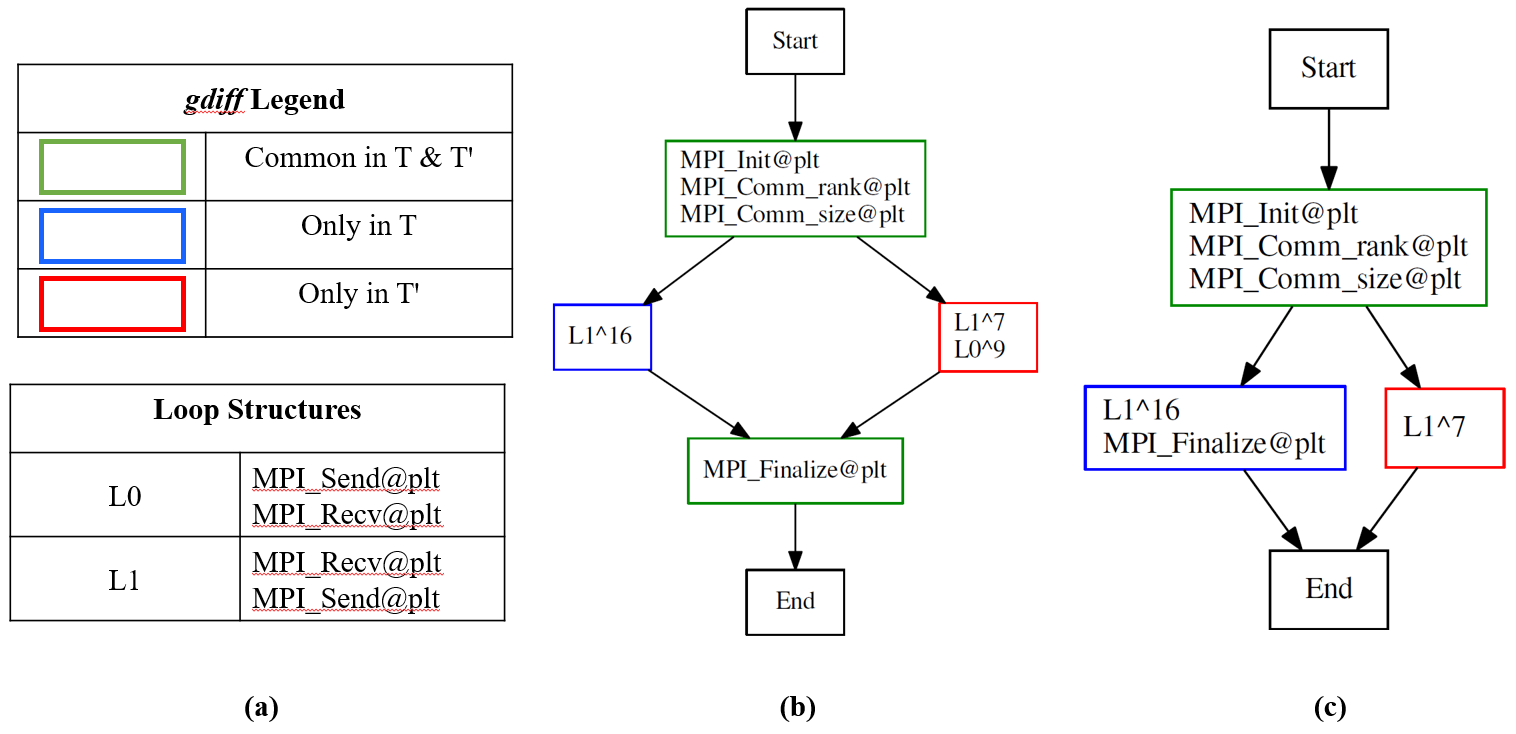
\includegraphics[width=0.45\textwidth]{figs/sampleGdiff.png}
\label{fig.gdiffs}
\end{figure}

%
We have planted two artificial bugs (\textit{swapBug} and \textit{dlBug}) in the code in figure \ref{fig.oddEven} and launched the code with 16 processes.
%
\textit{swapBug} swaps the order of MPI\_Send and MPI\_Recv in rank 5 after 7th iteration (of the loop in line 3 of \texttt{oddEvenSort}) simulating a potential deadlock and \textit{dlBug} simulates an actual deadlock (e.g., infinite loop) in the same location (rank 5 after 7th iteration).
%
Upon collection of ParLOT traces from execution above buggy versions, DiffTrace first decompresses traces and filters out all non-MPI functions.
Then two major loops are detected, \textbf{L0} and \textbf{L1}  (figure \ref{fig.gdiffs}-(a)) that are supposed to occur 16 times in even and odd ranks, respectively.
After analysis of CL models of execution, $x=5$ has been suggested as the most affected trace by the artificial bugs.
Figure \ref{fig.gdiffs}-(b) shows the 
\textit{gdiff}$(5)$ of \textit{swapBug} where $T_5$ iterates over the loop [MPI\_Recv - MPI\_Send] for 16 times (L1\^{}16) after the MPI initilization while the order swap has well reflected in $T_x^\prime$ (L1\^{}7 - L0\^{}9). Both processes seem to be terminated fine by executing MPI\_Finalize(). 
However, \textit{gdiff}$(5)$ of \textit{dlBug} (figure \ref{fig.gdiffs}-(c)) shows that while $T_5$ have executed MPI\_Finalize and terminated well, $T_5^\prime$ got stuck after executing L1 seven times and have never reached MPI\_Finalize.

This example shows that our approach can locate the impacted part of each execution by a fault. Having a pre-understanding of \textit{how the application should behave normally} would reduce the number of iterations by picking the right set of parameters on each pass. Relying on the knowledge of HPC developers, as the potential future users of DiffTrace, we believe our approach can post-mortem analyze of a ``dead'' execution and provides insight about "why the code died''.






%
%In the remainder of this section, we describe a chain of techniques that we apply to collected traces with having three main goals in mind:
%\begin{itemize}
%\item selectively pre-processing of traces to prune out uninteresting trace entries when we want to study a certain aspect of the dynamic behavior of the application. 
%\item reducing the search space by forming ``equivalent classes of traces'' and locating the trace or set of traces that got impacted the most by the fault.
%\item visualizing and reflecting the impact of fault to the potential faulty trace with respect to its corresponding fault-free trace.  
%\end{itemize}